\chapter{Funcionamiento del prototipo}

\section{Requerimientos}
El principal requerimiento a cumplir es la interacción con tarjetas RFID de acuerdo a la norma ISO14443, tanto para su lectura como escritura.
La comunicación con tarjetas de contacto de acuerdo a la norma ISO7816 es necesaria para la interacción con
un módulo de seguridad que permita la generación de las claves usadas para autenticarse
con las tarjetas RFID.
Por último mantener informado al usuario de lo que sucede durante una transacción
a través de una simple interfaz visual y sonora.


\section{Descripción del prototipo}
Este prototipo integra la lista de dispositivos que hoy en día se hacen llamar sistemas embebidos. Su hardware está integrado por una Single Board Computer (SBC), con un conversor de niveles de tensión (VLT), a la cual se conectan un lector/escritor de tarjetas RFID basadas en la norma ISO14443, un lector de tarjetas de contacto compatibles con la norma ISO7816, y la interfaz de usuario compuesta por un buzzer, leds y un display LCD16x2.
Entre las ventajas que podemos hallar en este dispositivo es que el lector/escritor de tarjetas RFID es un diseño realizado en PCB de dos capas que lo hace más sencillo y económico que el diseño del lector/escritor OpenPCD, y al igual que este último es compatible con la librería open source conocida como librfid.
Por su lado, en el lector de tarjetas de contacto debemos destacar su simplicidad, ya que no cuenta con ningún tipo de hardware específico (ASIC) que cumpla con el estandar ISO7816, sólo es necesario tener disponible un puerto serial (UART) y con un par de puertos de entrada/salida de propósito general para lo que tiene que ver con el manejo del oscilador y el reset para la tarjeta de contacto. Esto lo hace portable a cualquier SBC que cuente con los puertos detallados anteriormente.
Para la interfaz de usuario es necesario contar con siete puertos de entrada/salida de propósito general, para lo que es el control y la entrada de caracteres en el display, con cuatro puertos más para los leds y el buzzer.


\section{Funcionamiento general del prototipo}
Una vez que el prototipo $RF^{2}$ se encuentra operativo, el dispositivo despliega en el display el mensaje “Aproxime su tarjeta”, permaneciendo en dicho estado hasta que algún usuario acerque una tarjeta al lector/escritor RFID. 
En la primera transacción entre lector y tarjeta se obtiene el identificador único (UID) de ésta última, que será enviado al módulo de seguridad, SAM (previa autenticación exitosa), para que a partir de éste, se generen las claves de acceso que permitan la lectura y escritura de la tarjeta RFID.
Mientras se lleva a cabo la operación, se despliega en el display el mensaje, “No retire su tarjeta” a la vez que el led amarillo es encendido para indicar precaución ya que se están procesando datos.
La siguiente acción a llevar a cabo es verificar que la tarjeta del usuario tenga saldo pendiente de acreditar, en caso afirmativo se indica al usuario el saldo a acreditar a través del display con el mensaje “Saldo a acreditar \$...”. Si todo fue exitoso, se borra el saldo transferido de la lista de saldos pendientes a acreditar para que no se transfiera saldo indefinidas veces.
A continuación se despliega en el display el nuevo monto almacenado en la tarjeta, “Su saldo es de \$...”, se enciende el led verde y se emite un pitido mediante el buzzer en señal que la operación fue satisfactoria.
Por último se muestran en el display los mensajes “Transacción finalizada”, “Gracias” y vuelve al inicio para comenzar un nuevo ciclo.

En caso que la tarjeta no tuviera saldo pendiente de acreditar, el prototipo $RF^{2}$ funciona en modo consulta y despliega en el display el saldo disponible en la tarjeta, “Su saldo es de \$...”, encendiendo el led verde y emitiendo un pitido, seguido de los mensajes “Transacción finalizada”, “Gracias” y vuelve al inicio para comenzar un nuevo ciclo.

En caso de ocurrir un error durante alguno de los pasos anteriores, ya sea porque
el usuario retiró la tarjeta en un momento inadecuado, o simplemente porque el prototipo
no logró leer o escribir la tarjeta en forma correcta, se enciende el led rojo, se emite un
doble pitido mediante el buzzer, y el display muestra el mensaje “Error, vuelva a intentarlo”,
acto seguido el ciclo vuelve a comenzar. 

\bigskip
\begin{figure}[H]
\centering
  \begin{center}
   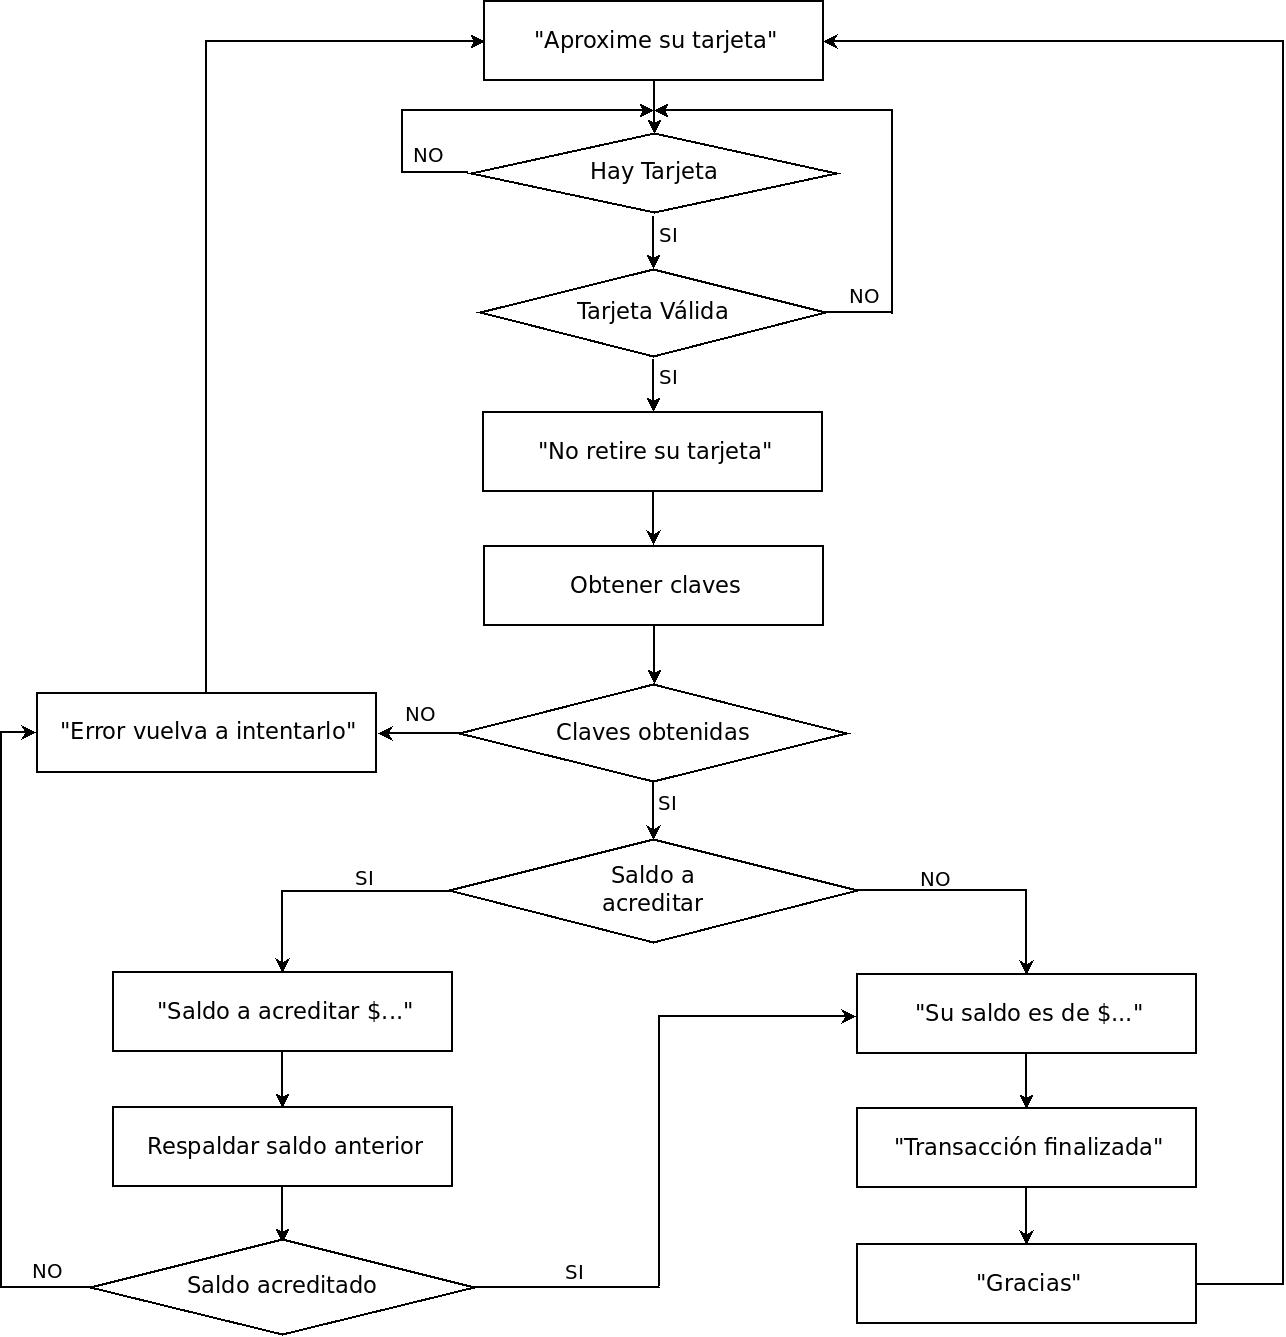
\includegraphics[scale=.35]{Imagenes/flujo.jpg}
  \end{center}
  \caption{Diagrama de flujo}\label{Fig:HW} 
\end{figure}